\section[]{Introduction} 

\plgic s are a family of essential proteins evolved for neuronal function in mammals. \plgic are gated by various neurotransmitters, but are functionally modulated by their boundary lipid composition. The well studied \plgic~\nachr conducts cations across the membrane to stimulate an action potential, and is functionally dependent on cholesterol and anionic lipids \citep{Dalziel1980,Ellena1983,M.CriadoH.Eibl1982,Fong1986,Fong1987,Jones1988a,Sunshine1994,DaCosta2009b}. Lipid binding sites for \plgic s are still relatively unknown.  Structural biology has predicted cholesterol and fatty acid binding sites in \plgic s \citep{Laverty2017,Basak2017}. Coarse grained molecular dynamics (CGMD) work by Sharp\citep{Sharp2019} and Woods\citep{Woods2019} predicted cholesterol binding sites around \nachr. \plgic-anionic lipid binding sites are still unknown. 

This work is the computational portion of a collaborative project analyzing \plgic~Erwinia ligand-gated ion channel's (ELIC) model boundary charged lipid composition using native mass spectrometry (NMS). Using CGMD as a computational microscope and simulating ELIC in membranes comprised of neutral 1-palmitoyl-2-oleoyl-sn-glycero-3-phosphocholine (POPC) and 1-palmitoyl-2-oleoyl-sn-glycero-3-phosphoethanolamine (POPE) and anionic 1-palmitoyl-2-oleoyl-sn-glycero-3-phosphoglycerol (POPG) we visualize and test potential anionic-ELIC binding distributions from NMS studies performed in \citep{Tong2019}. This work sought to determine 1) if charged phospholipids bound to ELIC, 2) determine where they bind, and 3) determine which sites modulate function.

\section[]{Computational Methods}
All simulations reported here used the MARTINI 2.2 \citep{DeJong2012} coarse-grained
topology and force field. The crystal structure of ELIC (PDB 3RQW) \citep{Pan2012}
was coarse-grained using MARTINI martinize.py script. Secondary
structural restraints were constructed using martinize.py while imposed
through Gromacs \citep{Berendsen1995}. Conformational restraints were preserved through
harmonic bonds between backbone beads less than 0.5 nm apart with a
coefficient of 900 kJ mol\textsuperscript{-1}. Pairs were determined
using the ElNeDyn algorithm \citep{Periole2009}. Membranes were constructed using the
MARTINI script insane.py \citep{Wassenaar2015}. The insane.py script randomly places
lipids throughout both inner and outer membranes and embeds selected
proteins into the membrane. Two series of simulations were developed,
the first using POPE and POPG, and the second POPC and POPG. Box sizes
were about 30 x 30 x 25 nm\textsuperscript{3} and each simulation box
contained about 3000 lipids.

Molecular dynamics simulations were carried out using GROMACS 5.1.4
\citep{Berendsen1995}. All systems were run using van der Waals (vdW) and electrostatics
in cutoff and reaction-field, respectively, with a dielectric constant
of $\epsilon = 15$. vdW and electrostatics used a cutoff length of
1.1 nm as defined in current MARTINI build specifications. Energy
minimizations were performed for about 30,000 steps. All systems were
run for short equilibration steps. Canonical ensembles (NVT) were run
for 100 ps using Berendsen thermostat set to 323 K with the temperature
coupling constant set to 1 ps. Isothermal-Isobaric ensemble (NPT)
equilibration was run for 5000 ps using Berendsen thermostat and
barostat. The thermostat was set to 323 K with the temperature coupling
constant set to 1 ps, and the barostat was set to a pressure coupling
constant of 3 ps with a compressibility of $3 x 10^{-5}$
bar$^{-1}$ holding at 1 bar. Molecular dynamics were
carried out using NPT ensemble and were simulated for 15 $\mu$s with a time
step of 0.015 ps using v-rescale thermostat set to 323 K and a
temperature coupling constant of 1 ps. Membranes consisting of POPE used
the Parrinello-Rahman barostat, and membranes consisting of POPC used
the Berendsen barostat, both under semi-isotropic coupling. The
reference pressure was set to 1 bar, the compressibility
3x10$^{-4}$ bar$^{-1}$, and the pressure
coupling constant 1 ps.

Annular lipids were determined using the annular lipid metric B:
\begin{equation}
    \begin{aligned}
    B_{i} = \left\langle \frac{b_{i}}{b_{\text{tot}}} \right\rangle\frac{1}{x_{i}} - 1
    \label{eq:B}
    \end{aligned}
\end{equation}

where $b_{i}$ is the instantaneous number of boundary lipids of
species $i$, $b_{\text{tot}}$ is the instantaneous total number of
boundary lipids, $x_{i}$ is the overall (bulk) fraction of species
$i$ and the brackets represent an average over time and replicas.
$B_{i} < 0$ and $B_{i} > 0$ indicate
enrichment and depletion of species $i$, respectively, relative to the
abundance in the bulk membrane. A given lipid was counted as a boundary
lipid if it was within 6 \AA of the ELIC transmembrane domain.

Two dimensional lipid density distributions around a central ELIC
pentamer were calculated for each leaflet using polar coordinates \citep{Sharp2019}.
For every sampled frame, all lipids of species $i$ were separated into
leaflets. For all $i$ lipids in a given leaflet, the vector separating
the phosphate beads from ELIC center was calculated and projected onto
the membrane plane. The two-dimensional separation vector was then used
to assign the lipid to the appropriate polar bin of radial bin width
$4\AA$ and angular bin width
$\frac{\pi}{15}$. The area density in each bin was averaged
over time and replicas.

\section[]{Computational Results}

To examine phospholipid interactions with ELIC using a molecular
model, coarse-grained MD simulations were performed on binary POPG/POPC
and POPG/POPE model membranes containing a single ELIC pentamer (Fig.
\ref{fig:Elic1}). Unlike fully-atomistic simulations, coarse-grained simulations
permit significant diffusion of lipids over simulation time scales. The
boundary lipid composition can thus equilibrate over the simulation
time, even if it varies significantly from the bulk membrane
composition. The POPG fraction was varied between 0 and 70\%. Enrichment
or depletion of POPG among boundary lipids for each concentration was
quantified using the boundary lipid metric B (Equation 3, see Methods).
For a given lipid species, $B>0$ reflects enrichment, $B<0$ reflects depletion, and B=0 reflects random mixing. For
POPG,$B>0$ for all compositions tested (Fig. \ref{fig:Elic1}B). This
result indicates that if POPG is present in the membrane, it is enriched
among boundary lipids. This enrichment is strongest for lower amounts of
POPG (i.e. lower $x_{\text{POPG}}$), consistent with specific binding
of POPG to ELIC.

\begin{figure}[htp]
	\center
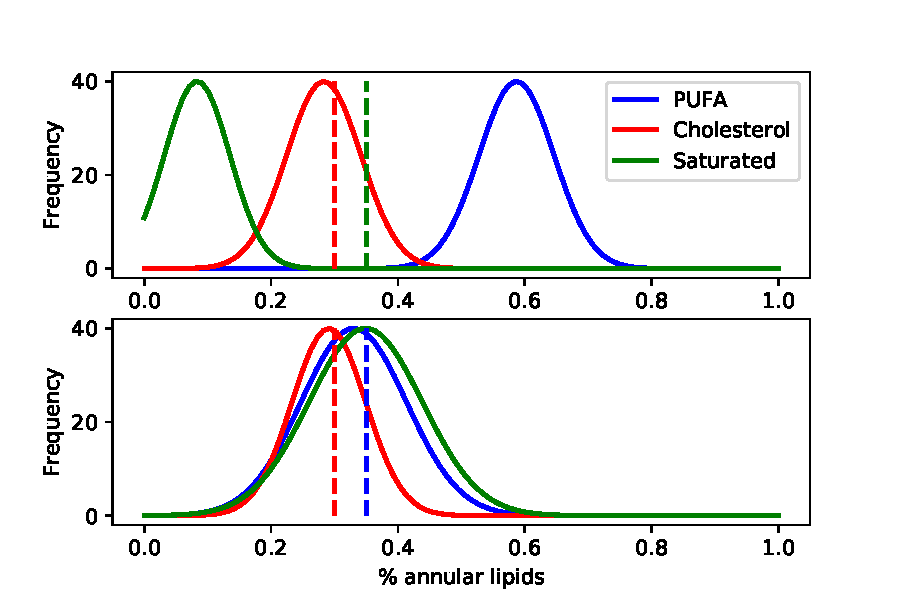
\includegraphics[width=.5\linewidth]{ELIC/Figure1.pdf}
\caption{Enrichment of POPG among ELIC boundary phospholipids from coarse-grained simulations. (A) Image of the simulation model of ELIC embedded in a membrane consisting of 10$\%$ POPG (pink) and $\%$ POPC (blue). The view is from the extracellular side of ELIC perpendicular to the membrane. (B) The boundary enrichment metric, B, is shown for phospholipid species in POPC/POPG membranes (left) or POPE/POPG membranes (right) over a range of POPG mole fractions $(x_PG)$. B is defined in Equation 3 (see Methods) and reflects the fractional difference between the amount of a lipid species found in the boundary and the bulk membrane: $B>0$ indicates enrichment, B<0 indicates depletion, and $B = 0$ indicates no difference in mole fraction between the bulk and the boundary. }
\label{fig:Elic1}
\end{figure}

We further examined these sites of interaction using our coarse-grained
MD simulations. To identify whether boundary POPG were localized around
specific helices or residues, two-dimensional densities of the
negatively-charged headgroup bead were calculated. The distributions are
separated by leaflet where each leaflet contained 10\% POPG. As shown in
Figure 5A, POPG was more likely to interact with ELIC in the inner
leaflet than the outer leaflet, consistent with three out of five
interfacial arginines residues being located on the intracellular
interface of the ELIC TMD. These three arginines are located on TM3
(R286) and TM4 (R299 and R301). Contacts between POPG and all three of
these residues are also visible in individual frames of the simulation
(Fig. 5B). Moreover, POPG is more likely to be contacting the
interfacial residues in TM4 (such as R299 and R301) than accessible
interfacial residues in any other helices (Fig. \ref{fig:Elic2}A). The remaining two
arginine residues are located at the TMD-ECD interface (R117 and R123).
POPG density in the outer leaflet localized to these residues at
intrasubunit sites between TM4 and TM1 or TM4 and TM3 (Fig. \ref{fig:Elic2}A), and
contacts between these residues and POPG headgroups in the outer leaflet
were also observed in snapshots from the MD simulations (Fig. \ref{fig:Elic2}B). In
summary, the native MS data and coarse-grained MD simulations
demonstrate that five interfacial arginines contribute to specific POPG
binding sites in the inner and outer leaflets adjacent to TM4.

\begin{figure}[htp]
	\center
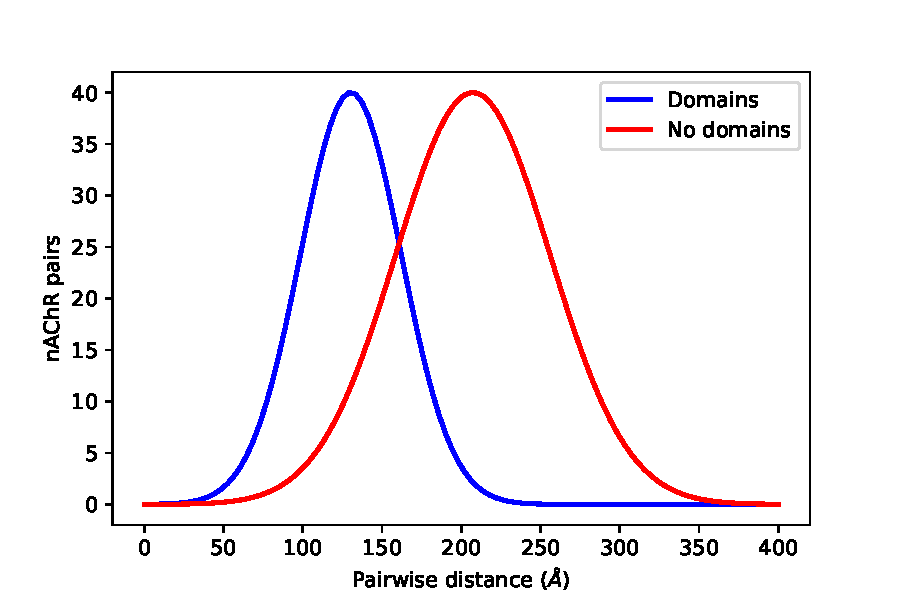
\includegraphics[width=\linewidth]{ELIC/Figure2.pdf}. 
\caption{Density calculations of lipids in binary membranes and visualization of direct POPG-ELIC interactions at $10\%$ POPG. (A) Distribution of POPG density in a POPG-POPC membrane, within 40 \AA from the ELIC pore over the last half of a 15 $\mu$s simulation, for both the outer leaflet (top) and the inner leaflet (bottom). Density is colored according to the color bar, where red and blue represent low and high POPG density, respectively. Circles represent the ELIC transmembrane backbone center of mass, with the helices containing the interfacial arginines colored in red (B) Representative frames after ~9 $\mu$s of simulation, showing multiple POPG binding modes associated with high density areas in (A). Two adjacent subunits of ELIC are shown in grey and white, while arginine side chains of interest are colored in peach, lime-yellow, orange, yellow, and red. POPG phosphate is colored in tan with the rest of the lipid in cyan.}
\label{fig:Elic2}
\end{figure}

\section[]{Summary}

This work sought to determine 1) if charged phospholipids bound to ELIC, 2) determine where they bind, and 3) determine which sites modulate function. NMS showed of the lipids POPC, POPE, and POPG, POPG consistently bound to ELIC more than either neutral lipid. Using CGMD we calculated the boundary enrichment of POPC, POPE, and POPG. We found POPG had the highest enrichment at the lowest concentration. This suggests specific binding sites for anionic lipids. Arginine residues at around the  TMD interfaces were hypothesized to be potential PG binding sites. Mutational studies, replacing positive arginine with polary neutral glutamine, in conjunction with NMS and electrophysiology, showed 1) less POPG bound and 2) a loss of function. CGMD density calculations predicted locations of high POPG density around inner intersubunit sites around ELIC's TMD. Each site contain 3 arginine. This suggests 1) anionic lipids bind to intersubunit sites, where positively charged arginine is, 2) mutating arginine to a polar neutral amino acid reduces anionic lipid binding, and 3) ELIC is functionally dependent on these arginines.
